% An End-to-End AI Agent for Kaggle Competitions
% Compile with pdfLaTeX (Overleaf default). No external assets required.
\documentclass[11pt,a4paper]{article}

\usepackage[margin=2.5cm]{geometry}
\usepackage{amsmath,amssymb}
\usepackage{newtxtext,newtxmath}
\usepackage{float}
\usepackage[section]{placeins}
\usepackage{booktabs}
\usepackage{caption}
\usepackage{microtype}
\usepackage{array}
\usepackage{enumitem}
\usepackage[hyphens]{url}
\usepackage[colorlinks=true, linkcolor=black, citecolor=black, urlcolor=blue!50!black]{hyperref}
\usepackage{xcolor}
\usepackage{tikz}
\usetikzlibrary{positioning,arrows.meta,calc,decorations.pathreplacing,shapes.geometric,fit}
% Figure role palette (draw.io convention used in the harness v1--v4 flowcharts)
\definecolor{flowblue}{HTML}{DAE8FC}\definecolor{flowblueline}{HTML}{6C8EBF}
\definecolor{flowgreen}{HTML}{D5E8D4}\definecolor{flowgreenline}{HTML}{82B366}
\definecolor{flowpurple}{HTML}{E1D5E7}\definecolor{flowpurpleline}{HTML}{9673A6}
\definecolor{flowgrey}{HTML}{F5F5F5}\definecolor{flowgreyline}{HTML}{999999}

\emergencystretch=1.5em

\captionsetup{font=small,labelfont=bf}
\newcolumntype{L}[1]{>{\raggedright\arraybackslash}p{#1}}
\renewcommand{\arraystretch}{1.15}
\newcommand{\dn}{\ensuremath{\downarrow}}
\newcommand{\up}{\ensuremath{\uparrow}}
% Agent abbreviations used in verdict columns
\newcommand{\M}{M}   % my-agent
\newcommand{\N}{N}   % NVIDIA
\newcommand{\A}{A}   % AIDE

\title{\textbf{An End-to-End AI Agent for Kaggle Competitions}\\
\large Benchmarked against two frozen yardsticks on 20 competitions\\
\normalsize\textcolor{orange!85!black}{Every printed number is a real measurement; all 20 benchmark lanes are complete, audited and scored.}}
\author{Wei-Hao Huang}
\date{}

\begin{document}
\maketitle

% =====================================================================
% PART: FRONT  --- abstract + Introduction
% Assemble immediately after \maketitle.
%
% TITLE BLOCK for the maintainer to place in the preamble, replacing the
% existing \title/\author/\date at source lines 38--42. Emitted here as a
% comment because this part file carries no preamble. The two subtitle
% lines and the orange status banner are dropped; their content is
% carried by the abstract and by the audit Results subsection.
%
%   \title{\textbf{Upstream problem identification, not downstream blending,\\
%   is where knowledge helps an autonomous\\
%   machine-learning agent}}
%   \author{Wei-Hao Huang}
%   \date{}
%
% The two explicit line breaks are load-bearing: without them the title
% sets as three lines with "agent" orphaned on the last. Verified by
% compiling the preamble + this title block.
% =====================================================================

\begin{center}\textbf{\large Abstract}\end{center}
\noindent Autonomous systems now run entire empirical pipelines, from raw dataset to scored
prediction, with no person in the loop. Where should external knowledge enter such a system? We
built one for machine-learning competitions and measured the answer. Downstream injection, among
the models being combined, moved scores by ${\sim}10^{-5}$ in our own implementation.
The agent therefore injects upstream, at problem identification: before any modelling it
classifies the task, how training and test periods relate, the validation split, and whether the
task needs data from outside the competition. Every verdict is scored on a real leaderboard,
judged by a paired test that reads each competition's noise off the two disjoint parts of its
test set.
Across 20 competitions the agent wins 16 of the 24 head-to-head comparisons in which it
separated from a rival by more than that noise ($66.7\%$), against $42.3\%$ for each of two frozen
reference agents, and takes the best held-out score on 10 of 20; 22 of the 60 comparisons cannot
be called at all. The upstream layer fires on exactly the 2 of 18
competitions that need external data and is silent on the other 16; all six controlled arms beat
their matched baselines; but no local signal we tested predicts which form the injection should
take. Placement of knowledge, not the amount of it, is what an autonomous pipeline can be
engineered around --- and a third of the comparisons being uncallable is itself the result that
any automated claim at this scale has to report.

\vspace{0.5em}

\section{Introduction}

Automated systems increasingly run a whole empirical study rather than one step of it: from a
raw dataset, through the choice of how to validate, to a result that will be judged. Three
things a human investigator normally supplies then pass to the machine. The first is judgment
about the problem: deciding what kind of task this is and what it needs, before any tuning
begins. The second is measurement: knowing whether a claimed improvement exceeds the noise of
the instrument that produced it. The third is the honesty of the claim: whether the system's own
checks can catch its own contamination, and whether those checks can themselves be caught being
wrong. Machine-learning competitions are one of the few settings in which all three are
externally scorable: a hidden test set held by a third party, a single scalar score, and
thousands of human teams fixing the scale of what counts as good.

Recent agents exploit that property. AIDE searches a tree of complete candidate solutions,
mutating each on the error or score it returns~\cite{aide2025}. ERA couples a language-model
rewriter with tree search and externally injected research ideas, outperforming strong baselines
across 16 Kaggle Playground competitions~\cite{aygun2026}. Industrial agents skip search
altogether and reproduce the strongest public solution to the competition at
hand~\cite{nvidia2026}. Each embodies a different answer to where knowledge should enter the
pipeline; none tests its answer against the alternatives.

An agent's own cross-validation cannot arbitrate between agents. It is not a leaderboard proxy
--- on one competition here a pooled out-of-fold SMAPE of $6.706$ sat against a realized
leaderboard score of $49.40878$ --- and it is computed on a split the agent itself chose, which is
part of what is under test. External scores are not self-interpreting either: in the development
runs behind this study the top-two private gaps sat at the fourth and fifth decimal place
($0.00003$; $0.00000$), and rerunning an agent unchanged moves its score by a comparable amount.
We therefore score every verdict on the real leaderboard and adjudicate it with an error model
taken from the data: Kaggle splits each test set into two disjoint subsets, public and private,
and one submission receives a score on each, so how far a between-agent gap moves across the two
subsets measures that competition's own noise.

\textbf{my-agent} runs the full loop --- problem identification, exploratory analysis, feature
engineering, modelling, evaluation, submission --- with a language model reasoning at every stage
and gradient-boosting libraries invoked through the shell. Three mechanisms distinguish it: a
cross-competition experience library in which every stored insight must carry a score delta as
its evidence; a tree search in which ensembles are first-class nodes over cached out-of-fold
predictions (37--224 evaluated nodes per competition); and a stage that identifies the problem
from the competition statement and data schema, before any analysis. That stage carries the design decision. Our first answer was the
conventional one --- inject downstream, among the candidates being blended --- and measuring our
own implementation showed it worth ${\sim}10^{-5}$. Knowledge therefore enters upstream:
the stage writes a structured dossier of task family, train--test window relation, split policy
and external-data need, and emits typed operators into a whitelisted, leakage-guarded
external-data module.

An architectural claim needs reference points we did not build and cannot tune. We froze two
methodologically distinct yardsticks --- \textbf{AIDE}, tree search with no cross-competition
memory, and the \textbf{NVIDIA Kaggle Agent}, which reproduces the highest-voted public kernel
--- and improved neither, even where we found weaknesses. All three ran on 20 tabular
competitions, and on three further competitions spanning language pairing, physiological time
series and dermoscopic imaging, one lane at a time on one machine under mechanically enforced
isolation. my-agent's benchmark lanes held no credentials, so no lane could consult a
leaderboard or submit; a separate operator step scored the frozen submissions, and every lane's
tool-call transcript was audited before its score was accepted.

my-agent leads the resulting standing under an adjudication rule fixed before any score
existed, and the upstream layer separates cleanly across the task distribution while winning
every controlled arm we ran. Both results come with a boundary the same measurement draws: a
third of the comparisons cannot be called at the noise scale of the leaderboards themselves, and
where the agent loses it loses to faithful reproduction of an existing public solution rather
than to a better search. The hypothesis we cared about most failed outright --- no local signal
we tested selects which form an injection should take --- and we report it here as a result,
because a method that cannot kill its own hypotheses is not measuring anything.


% ============================================================================
%  PART: RESULTS  (Nature-style rewrite of REPORT_v6.tex)
%  Assembled between the Introduction and the Discussion.
%  Main-text display items defined here: Fig. 1 (fig:arch),
%  Table 1 (tab:injection), Table 2 (tab:winrates), Table 3 (tab:midcx).
%  Labels defined here: sec:exp4, sec:votes, sec:exp5v5, sec:exp6v5,
%  sec:winrates, sec:reversal, sec:rerun, sec:exp7run2.
%  Labels referenced from elsewhere: sec:v5, sec:apparatus, sec:exp2,
%  sec:fairness, sec:exp1, sec:limitations, sec:future, fig:tree, tab:bench,
%  tab:comps, tab:nodes, tab:drift, tab:variance, tab:splits, tab:threeway,
%  app:specs, app:coverage.
% ============================================================================

\section{Results}

\subsection{An agent that classifies the problem before it models it}

my-agent commits to a classification of the problem from the competition statement and the
data schema alone, before any analysis or modelling, and every mechanism that distinguishes it
from the two yardsticks hangs off that commitment. Execution
runs through six stages --- data ingestion, Stage 0.5 problem dossier, exploratory data
analysis (EDA), feature engineering, modelling, evaluation, submission --- with an LLM (Claude
Code) reasoning and deciding at each one, and with LightGBM, XGBoost, CatBoost and Optuna
invoked through the shell for model fitting, hyperparameter search and ensembling
(Fig.~\ref{fig:arch}). Stage 0.5 answers four questions before any modelling begins --- task
family, train--test window relation, split policy, external-data need --- and writes them to a
structured dossier. The dossier is a prior, not a conclusion: EDA must test its hypotheses and
record a verdict against it.

Three mechanisms hang off that stage. A cross-competition experience library supplies priors
and is gated on evidence: every entry must carry a competition, an experiment number and a
score delta, and entries without one are rejected. Neither reference method carries
cross-competition memory, and this study does not measure what the library itself contributes:
no ablation of it was run, so the standing below cannot be attributed to it. An external-data layer
realises the dossier's data-level operators as whitelisted, leakage-guarded joins, each raced
against a no-external baseline inside the search. And a tree search over candidate solutions is
the optimisation loop: each node is a complete, executable solution scored by local
cross-validation, lineages are abandoned on plateau, and ensembles are first-class node kinds
built over cached out-of-fold predictions with weight search, so blend nodes compete with solo
nodes for the global best rather than being assembled once at the end (Extended Data
Fig.~\ref{fig:treeex}). Lanes evaluate 37--224 nodes per
competition against a default budget of 60, extended through a documented resume path
(Table~\ref{tab:nodes}). The agent takes one linear pass to a validated single model and a
first blend before switching to search; internal development evaluation had tree search winning
9 of 10 competitions with 1 tie and 0 losses against that linear protocol, and every benchmark
lane used it.

The pipeline also documents itself. Each lane records a structured EDA pass --- distributions,
drift, correlation --- into machine-readable records and emits no image files; every
experiment's parameters, features, split scheme and scores are logged in structured form, so
every number in this paper traces to a logged run; and a reporting layer renders those records
into a five-section per-competition specification report, 22 for my-agent and 17 re-documenting
the AIDE runs under the same framework (Appendix~\ref{app:specs}). A benchmark lane holds no
Kaggle credentials, runs alone on the machine, reads only its own validated data root, freezes
a submission file, and has every tool call it made read afterwards by a transcript audit;
scoring is a separate credentialed operator step (Section~\ref{sec:apparatus}).

\begin{figure}[htbp]
\centering
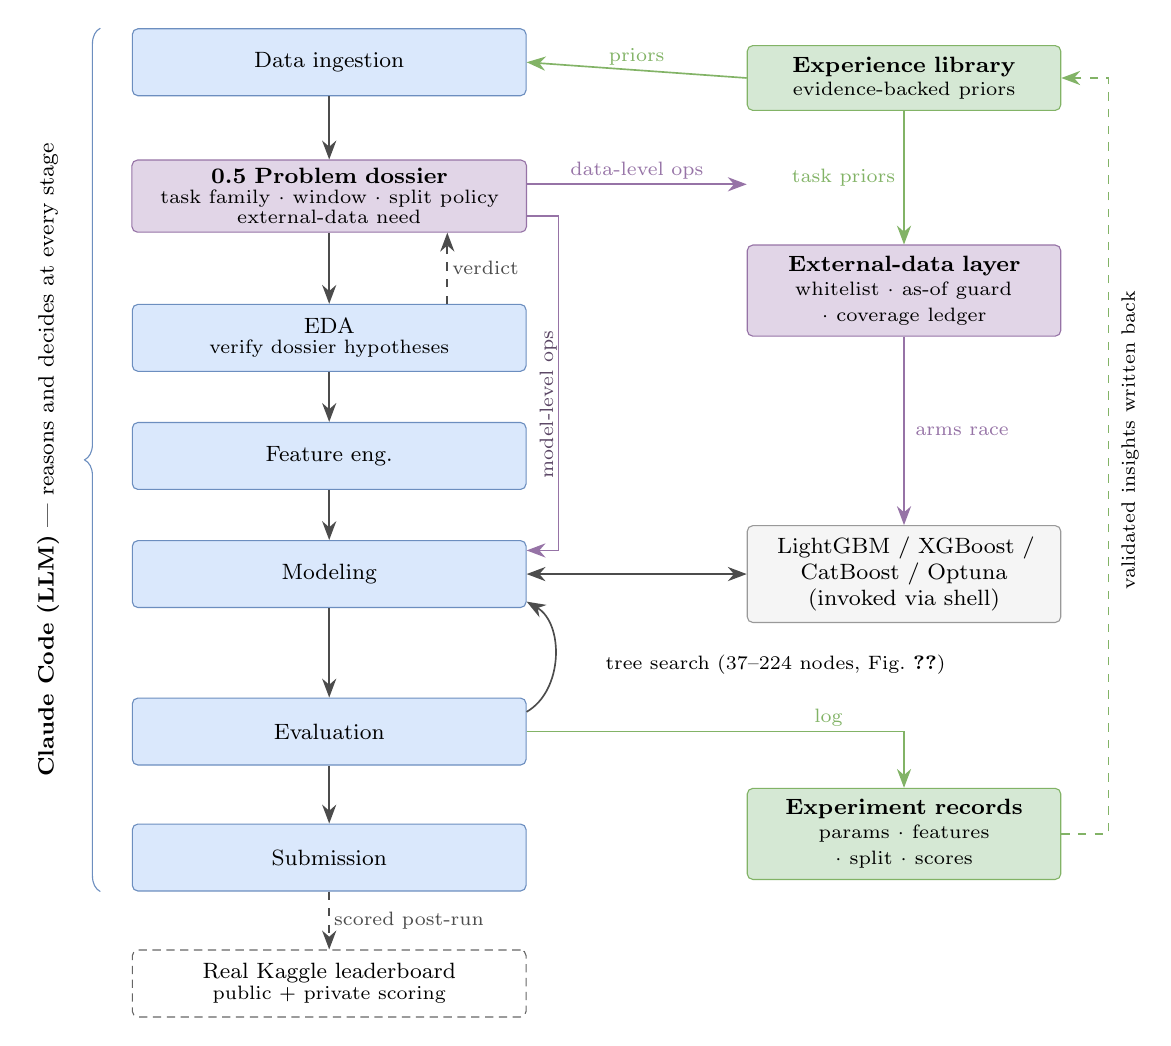
\begin{tikzpicture}[
  font=\footnotesize,
  stage/.style={draw=flowblueline, rounded corners=2pt, align=center, inner sep=3pt,
                fill=flowblue, minimum height=8.5mm, minimum width=50mm},
  inj/.style={stage, fill=flowpurple, draw=flowpurpleline},
  supp/.style={draw=flowgreenline, rounded corners=2pt, align=center, inner sep=4pt,
               fill=flowgreen, text width=37mm},
  injbox/.style={supp, fill=flowpurple, draw=flowpurpleline},
  toolbox/.style={supp, fill=flowgrey, draw=flowgreyline},
  arr/.style={-{Stealth[length=2.4mm]}, semithick, black!70},
  parr/.style={arr, flowpurpleline},
  garr/.style={arr, flowgreenline},
  darr/.style={arr, dashed},
  lab/.style={font=\scriptsize, inner sep=1.5pt}
]
% ----- main pipeline (top -> bottom) -----
\node[stage]              (s1)  at (0,0)     {Data ingestion};
\node[inj, text width=48mm] (s05) at (0,-1.7)
  {\textbf{0.5 Problem dossier}\\[-1pt]
   {\scriptsize task family $\cdot$ window $\cdot$ split policy\\[-2pt]external-data need}};
\node[stage]              (s2)  at (0,-3.5)  {EDA\\[-2pt]{\scriptsize verify dossier hypotheses}};
\node[stage]              (s3)  at (0,-5.0)  {Feature eng.};
\node[stage]              (s4)  at (0,-6.5)  {Modeling};
\node[stage]              (s5)  at (0,-8.5)  {Evaluation};
\node[stage]              (s6)  at (0,-10.1) {Submission};
\foreach \a/\b in {s1/s05, s05/s2, s2/s3, s3/s4, s4/s5, s5/s6}{\draw[arr] (\a) -- (\b);}
% ----- EDA verdict back to the dossier -----
\draw[darr] ([xshift=15mm]s2.north) -- node[lab, right]{verdict} ([xshift=15mm]s05.south);
% ----- pipeline endpoint: the real leaderboard -----
\node[stage, densely dashed, fill=white, draw=black!60] (lb) at (0,-11.7)
  {Real Kaggle leaderboard\\[-2pt]{\scriptsize public + private scoring}};
\draw[darr] (s6) -- node[lab, right]{scored post-run} (lb);
% ----- LLM annotation: vertical brace spanning all stages -----
\draw[decorate, decoration={brace, amplitude=2mm}, flowblueline]
  ([xshift=-4mm]s6.south west) -- ([xshift=-4mm]s1.north west)
  node[midway, xshift=-4mm, rotate=90, anchor=south, black]
  {\textbf{Claude Code (LLM)} --- reasons and decides at every stage};
% ----- tree-search loop (Evaluation -> Modeling), arc in the corridor -----
\draw[arr] ([yshift=2.5mm]s5.east) to[out=30, in=-30] ([yshift=-3.5mm]s4.east);
\node[lab, anchor=west] at (3.45,-7.65) {tree search (37--224 nodes, Fig.~\ref{fig:tree})};
% ----- right rail -----
\node[supp]    (lib)   at (7.3,-0.2)  {\textbf{Experience library}\\[-1pt]
  {\scriptsize evidence-backed priors}};
\node[injbox]  (ext)   at (7.3,-2.9)  {\textbf{External-data layer}\\[-1pt]
  {\scriptsize whitelist $\cdot$ as-of guard $\cdot$ coverage ledger}};
\node[toolbox] (tools) at (7.3,-6.5)  {LightGBM / XGBoost /\\CatBoost / Optuna\\(invoked via shell)};
\node[supp]    (rec)   at (7.3,-9.8)  {\textbf{Experiment records}\\[-1pt]
  {\scriptsize params $\cdot$ features $\cdot$ split $\cdot$ scores}};
% ----- rail / pipeline connections -----
\draw[garr] (lib.west) -- node[lab, above]{priors} (s1.east);
\draw[garr] (lib.south) -- node[lab, anchor=east, xshift=-0.5mm]{task priors} (ext.north);
\draw[parr] ([yshift=1.5mm]s05.east) -- node[lab, above]{data-level ops}
  ([yshift=1.5mm]ext.west |- s05.east);
% ----- model-level operators: dossier seeds the search directly -----
\draw[parr] ([yshift=-2.5mm]s05.east) -- ++(4mm,0) |- ([yshift=3mm]s4.east);
\node[lab, rotate=90, anchor=south, flowpurpleline!60!black] at (2.95,-4.35)
  {model-level ops};
\draw[parr] (ext.south) -- node[lab, anchor=west, xshift=0.8mm]{arms race} (tools.north);
\draw[arr, {Stealth[length=2.4mm]}-{Stealth[length=2.4mm]}] (s4.east) -- (tools.west);
\draw[garr] (s5.east) -- node[lab, above, pos=0.8]{log} (rec.north |- s5.east) -- (rec.north);
% ----- dashed write-back, up the far right -----
\draw[darr, flowgreenline] (rec.east) -- ++(6mm,0) |- (lib.east);
\node[lab, rotate=90, anchor=north] at (10.0,-4.8) {validated insights written back};
\end{tikzpicture}
\caption{Architecture of my-agent. Color marks role.
\textbf{Blue --- the LLM-driven pipeline}: Claude Code reasons and decides at every stage;
EDA verifies the dossier's hypotheses and records a verdict (the dossier is a prior, not a
conclusion). \textbf{Purple --- the injection layer} (Section~\ref{sec:v5}): the Stage-0.5
dossier classifies the task from the problem statement and task-\emph{type} priors only (no
competition kernels) and emits typed operators --- data-level operators drive the
external-data layer (whitelisted sources, leakage-guarded as-of joins, a
proposed/realized/unrealized coverage ledger), whose arms race against a no-external
baseline with the winner taking the full budget, while model-level operators seed search
lineages directly. \textbf{Green --- the evidence loop}: the experience library (every entry
carries score-delta evidence; queried before EDA and modeling) and the experiment records
that log every run's params, features, split, and scores, with validated insights written
back. \textbf{Gray --- Auto-ML tools} invoked via the shell. Solid arrows: the forward
execution flow; dashed arrows: feedback, advisory, or post-run steps outside it (the
verdict, the write-back, leaderboard scoring). The leaderboard is external to
the agent: lanes hold no credentials, and submissions are scored only after the run.}
\label{fig:arch}
\end{figure}


\subsection{Downstream injection is worth about $10^{-5}$; the gap all three agents share is upstream}
\label{sec:exp4}

Our first design put external knowledge downstream, among the candidates being blended, and
measuring it showed that placement to be worth almost nothing. Reweighting never displaced the
convex-optimum champion in 8 of 8 rigorous competitions, and expanding the candidate pool
helped 2 of 8 by about $10^{-5}$. We abandoned that placement; no benchmark submission in this
paper uses it.

Reading the three agents' development-run execution logs and champion code relocated the gap
upstream, to problem-level judgment rather than tuning skill. AIDE can diagnose a problem but
has no mechanism that lets a diagnosis veto a score: on s3e19 it accidentally swapped its
time-based validation for shuffled KFold mid-run, its metric instantly ``improved'' from
$18.42$ to $4.41$ --- an optimism a controlled split-only experiment measures at $4.5\times$
(Table~\ref{tab:splits}) --- and it tuned against the leaked number to the end, while my-agent
quarantined the same split as diagnostic only.
\label{sec:votes}%
The NVIDIA agent reproduced its source kernel's skeleton on the same competition but missed the
step that decides the outcome, and its selection signal --- the vote count of a public kernel
--- measures popularity rather than quality, with nothing in the method checking the reproduced
score against the source's claimed rank. All three agents missed the same thing on s3e19: the
task needs external data. At matched budget the per-country GDP join used by the leaderboard's
better half is worth about $6$ SMAPE of a ${\sim}44$-point gap, the remainder being a
full-future-year extrapolation that defeats every method in the comparison equally. The
upstream layer is the architectural answer to exactly this class of miss.

\subsection{The dossier fires on the tasks that need external data and is silent on the rest}
\label{sec:exp5v5}

Run as a classifier over the task distribution, the problem dossier separates cleanly: it fires
on exactly the 2 of the 18 original benchmark competitions that need external covariates and
reports ``no'' or ``unlikely'' on the other 16. The two it fires on are the country-panel time
series s3e19 and tps-jan-2022, whose accepted solutions are known to require external
covariates; the 16 silences cover the i.i.d.\ tabular, categorical, spectral and
structured-output tasks (Table~\ref{tab:comps}). Sensitivity is therefore 2/2 and specificity
16/16, obtained from the problem statement, the data schema and task-\emph{type} priors alone,
in minutes per competition and with no training.

Two caveats bound that claim, and they cut in opposite directions. The sensitivity half is
partly in-sample: the task priors the dossier reads were distilled from this benchmark's own
failure analysis of exactly those two competitions, so 16/16 is the informative half, and 2/2
carries a 95\% confidence interval reaching down to 16\%. The two firing-class competitions
added later (s5e1, tps-sep-2022) also fire, but they were \emph{selected} as firing-class, so
the sweep claim rests on the original 18. Two secondary behaviours are worth recording. On
s3e19 the dossier surfaced a genuine conflict --- a conservative setup-time \path{config.yaml}
flag said external data was not allowed while the task prior's evidence implied otherwise ---
and flagged it for verification rather than guessing (the official rules, Section 7.C, settle
it in favour of permission). On the out-of-scope SIIM imaging task it answers ``no'', which is
correct within the current source whitelist, whose classes do not yet include prior-competition
archives.

\subsection{All six controlled external-data arms beat their baselines}
\label{sec:exp6v5}

Every controlled arm the layer produced beat its matched baseline, and each margin passes the
paired public--private test. Across the three firing-class competitions --- s3e19, the
benchmark's canonical failure and the causal test bed; tps-sep-2022, a held-out replication
with the dossier written in advance; and s5e1, a pre-registered test --- all six external-data
arms beat their no-external baselines, every one paired-significant. Arms were built so that
the operator's added columns are the only difference from the baseline, verified digit-identical
otherwise, and every arm was submitted for real public and private scores. In matched
configuration the feature join is worth $6.01$ private SMAPE on s3e19 and $2.09$ on the
held-out tps-sep-2022; at a full 46-node search budget per arm both external arms still beat
the searched baseline, so the effect is not an artefact of a starved control; and on s5e1 the
winning form takes a $20\%$ relative private-MAPE margin ($0.12417$ against $0.15751$), the
largest effect in the class.

On the canonical failure itself, a with-layer/without-layer ablation --- the full pipeline
against a searched champion from the identical pipeline with the layer disabled --- passes the
paired test: private $48.243$ against $50.455$, with $d_{\mathrm{pub}}=+3.389$,
$d_{\mathrm{priv}}=+2.212$ and a gap movement of $1.177$, so the gap comfortably exceeds its
own movement across the two test subsets. That with-layer champion sits numerically ahead of
both frozen yardsticks on s3e19 ($48.26558$ and $48.34131$). It is a controlled arm and not the
benchmark s3e19 lane, which ran without the layer and scored $49.40878$; we make the comparison
in Table~\ref{tab:injection} rather than in the benchmark table for that reason.

\begin{table}[t]
\centering\small
\setlength{\tabcolsep}{4pt}
\caption{What the upstream injection layer fires on and what it delivers. Every row is a
measurement on real competition data. Controlled arms differ from their baseline only in the
operator's added columns, verified digit-identical otherwise, and each was submitted for real
public and private scores; ``paired-significant'' means the gap replicates in sign across the
public and private test subsets and exceeds its own movement between them. Lower is better for
SMAPE and MAPE. $^{\ast}$The ablation figures are controlled arms, \emph{not} the benchmark
s3e19 lane, which ran without the layer and scored $49.40878$ (Table~\ref{tab:bench}).}
\label{tab:injection}
\begin{tabular}{@{}L{4.0cm}L{4.7cm}L{5.9cm}@{}}
\toprule
\textbf{Measurement} & \textbf{Setting} & \textbf{Result} \\
\midrule
Dossier sensitivity & 18 original benchmark competitions; problem statement, schema and task-type priors only; no training & Fires on 2/2 competitions needing external data \\
Dossier specificity & same 18 competitions & Silent on 16/16 competitions not needing it \\
\addlinespace[2pt]
External-data arms & 3 firing-class competitions, matched configuration, real submissions & \textbf{6 of 6} beat their baseline; every one paired-significant \\
Matched join, s3e19 & operator columns the only difference & $6.01$ private SMAPE \\
Matched join, tps-sep-2022 & held-out replication, dossier written in advance & $2.09$ private SMAPE \\
Winning form, s5e1 & pre-registered test & $0.12417$ vs.\ $0.15751$ private MAPE ($20\%$ relative) \\
\addlinespace[2pt]
With-layer vs.\ without-layer ablation, s3e19$^{\ast}$ & full pipeline vs.\ searched champion of the identical pipeline, layer disabled & private $48.243$ vs.\ $50.455$; $d_{\mathrm{pub}}\,{+}3.389$, $d_{\mathrm{priv}}\,{+}2.212$, movement $1.177$ \\
\addlinespace[2pt]
Form selection (negative) & cross-validation, held-out-year protocol, proportionality diagnostic & \textbf{0 of 3} rank the form verdict correctly; the survivor's pre-registered falsifier fired \\
Consumer trace (negative) & 241 ideas proposed across 20 dossiers & $73\%$ expressible as an operator; $5\%$ actually consumed at first measurement, $27\%$ after wiring a consumer \\
\bottomrule
\end{tabular}
\end{table}

\subsection{Two things the layer cannot do, measured}

No local signal we tested selects which \emph{form} the injection should take. Cross-validation,
a held-out-year protocol and a proportionality diagnostic each misrank the form verdict, 0 for
3. The proportionality diagnostic was the one selector that survived hindsight, so we put it to
a pre-registered test on s5e1, committing its prediction to version control before any model
was fitted; its named falsifier fired. The layer therefore races both forms inside the search,
always, rather than choosing between them, and the one surviving post-hoc candidate --- horizon
length --- is committed as a pre-registration binding the next firing-class competition before
its leaderboard is consulted (Section~\ref{sec:future}). This is a negative result with a price
attached: the form choice was worth more than the entire search budget on one competition and a
$20\%$ relative margin on another.

The second limit is that proposing an idea is not the same as using it, and our own accounting
initially could not tell the difference. Across the 20 dossiers the layer proposes 241 ideas.
Counting those whose operator family exists gives $73\%$; tracing which are actually
\emph{consumed} by a search driver gave only $5\%$ at first measurement, because the three
operators supplying most of the higher figure were emitted into a key that no search driver
read, while the dispatcher recorded them as realized. Wiring a consumer and moving the
target-free encodings into the data layer raised the traced figure to $27\%$. A produced
artifact with no consumer is indistinguishable from a working one in every log, score table and
coverage metric --- and this instance occurred inside the very mechanism built to prevent
silent truncation. An architecture claim needs a consumer trace, not a vocabulary count
(Appendix~\ref{app:coverage}).

\subsection{my-agent leads the three-agent standing, and a third of the duels are undecidable}
\label{sec:winrates}

Under the paired error model, my-agent wins 16 and loses 8 of its 24 decided duels ($66.7\%$),
against $42.3\%$ for each of the two frozen yardsticks, which win 11 and lose 15 of their own
26. The evaluation set gives 20 competitions $\times$ 3 pairings $=$ 60 duels, and with all 20
lanes scored every one of them is adjudicated: 38 produce a verdict and 22 do not. The 22 are
not ties. Nineteen fail the requirement that the ordering replicate in sign across the public
and private test subsets, or that the gap exceed its own movement between them; three die on a
per-competition between-run variance floor. The win-rate denominators differ between agents
(24 for my-agent, 26 for each yardstick) because a duel is decided or not independently for
each pair. Table~\ref{tab:winrates} gives the standing; per-competition scores are in
Table~\ref{tab:bench}.

The three floor kills are worth naming individually, because each removes a verdict a raw
reading would have awarded: s3e16 and s5e10 would have been my-agent wins, and s6e2 an AIDE win
(private gap $0.00011$ against AIDE's measured $0.00020$ wobble there; Table~\ref{tab:variance}).
s5e10 is the sharpest case. The private gap between my-agent and AIDE is
$|d_{\mathrm{priv}}| = 0.00003$, exactly equal to AIDE's measured between-run wobble on that
competition. The rule requires the gap to \emph{exceed} the floor, and we compare in exact
decimal, so the duel stays undecidable rather than becoming a seventeenth my-agent win --- a
case the error model flagged in advance, before the benchmark scores existed.

Two readings that the paired test does not replace sit alongside it. On the raw,
direction-aware comparison of private scores, my-agent takes the best of the three on 10 of the
20 competitions, NVIDIA on 7 and AIDE on 3, with no ties anywhere; and my-agent's benchmark
submission beats its own development-lane private score on 13 of 20, so the frozen, audited,
credential-free rerun is not a weakened version of the development runs. As an absolute
reference, NVIDIA's median percentile rank against the frozen final leaderboards is 68.0 (range
$18.8$--$96.5$) and AIDE's is 68.7 ($26.4$--$97.9$); my-agent's percentile ranks require a
leaderboard-snapshot pull and are not reported here.

\begin{table}[htbp]
\centering\small
\caption{Standing of the three agents on the 20-competition benchmark. Each competition
contributes three duels, one per pair of agents, giving 60 duels, all adjudicated: 38 decided
and 22 undecidable. The 22 undecidable duels are \emph{not} ties --- 19 fail the
sign-agreement or gap-stability condition of the paired public--private test, and 3 fall below
a per-competition between-run variance floor. Win rate is over each agent's own decided duels
(my-agent 24, each yardstick 26), which is why the denominators differ. ``Best private score''
counts competitions on which that agent's private leaderboard score is the best of the three on
a raw, direction-aware reading; there are no ties. Percentile rank (PR) is the share of a
competition's final private standings the submission would beat, a would-be rank $r$ among $N$
teams giving $\mathrm{PR}=100\,(N-r)/N$ against the frozen final leaderboard.}
\label{tab:winrates}
\begin{tabular}{@{}lrrrrl@{}}
\toprule
\textbf{Method} & \textbf{Wins} & \textbf{Losses} & \textbf{Win rate (decided duels)} &
\textbf{Best private score} & \textbf{Median PR (range)} \\
\midrule
my-agent & 16 & 8  & 66.7\% & 10 of 20 & not available$^{\ast}$ \\
NVIDIA   & 11 & 15 & 42.3\% & 7 of 20  & 68.0 (18.8--96.5) \\
AIDE     & 11 & 15 & 42.3\% & 3 of 20  & 68.7 (26.4--97.9) \\
\bottomrule
\end{tabular}

\smallskip
\raggedright\footnotesize
$^{\ast}$~my-agent's percentile ranks require a leaderboard-snapshot pull and are not reported.
\end{table}

\subsection{my-agent's losses fall where a mature public solution already exists}
\label{sec:reversal}

my-agent's two sharpest losses are the two benchmark competitions that have a mature,
high-quality public solution, which is where faithful reproduction beats autonomous search. On
tps-sep-2022 it scores $28.49605$ SMAPE against $5.48351$ for NVIDIA and $9.72095$ for AIDE; on
tps-jan-2022 it scores $6.29895$ against NVIDIA's reproduction of the known GDP-ratio solution
at $4.63651$. Neither gap is anywhere near the measurement noise the error model absorbs:
my-agent's own public and private scores on tps-sep-2022 are $28.45070$ and $28.49605$, so the
sampling noise there sits in the second decimal place while the gap it loses by runs to whole
SMAPE points. Search wins the rest of the set, which is dominated by obscure,
build-your-own-pipeline tasks with no such solution to copy.

The same reversal appears inside a single competition. On s5e1 the public half of the test
split favours NVIDIA and the private half favours my-agent, so that duel fails the
sign-agreement condition and is undecidable by construction rather than by any shortage of
signal --- the development-lane case replicated live in the frozen run. The standing is
correspondingly sensitive to which competitions are in the set: dropping s3e19 alone takes
my-agent from $66.7\%$ to $72.7\%$, and dropping s3e3 takes NVIDIA from $42.3\%$ to $37.5\%$.

\subsection{The audit gate fires in both directions, and our own auditor was blind at its target}
\label{sec:rerun}

An audit is evidence only if it can discard a result that flatters us and can itself be caught
being wrong; ours did both. All 20 lanes completed, were transcript-audited and were scored,
over roughly 26 hours of accepted lane attempts. The queue halted three times: twice on the
same environment fault and once on the rule that stops the whole queue after two consecutive
audit failures. That environment fault was ours rather than the method's --- the sandbox bound
the session credential file read-only, so a lane whose access token expired mid-run could not
write the refreshed token back and died with an authentication error, 39 and 75 minutes in. We
fixed it after the benchmark with a writable bind and a budget-aware preflight that refuses to
start a lane whose token cannot outlive it.

The gate fired hardest on s3e19. Its first attempt opened the raw knowledge library four times,
bypassing the query interface's self-citation exclusion, and the audit discarded it. The clean
re-run scores \emph{worse} on local cross-validation --- pooled out-of-fold SMAPE $6.706$
against the tainted attempt's $5.740$ --- consistent with the contamination advantage being
real and the audit pricing it correctly. A benchmark that discards a better-looking number and
keeps the honest one has evidence its audit does something. The same transcript also tripped
the network detector; re-reading it showed the hit to be a Python variable named \texttt{nc}
inside a diagnostic heredoc, so the four raw-library opens carry the discard on their own.

The recurrence, not the individual incident, is the finding. Four of the twenty lanes wrote
their own library write-back script, because the skill instructs every lane to write validated
insights back through library tools this run root does not ship, and the root bound the shared
library writable so that a lane could write its own workspace. That is a fault of the harness
rather than of any lane, and only one instance of it crossed lanes: tps-aug-2022 wrote three
insights back minutes after finalising its submission, tps-jan-2022 started two minutes later
and its Stage 0.5 read served the polluted entries, so we killed that lane at one minute,
reverted the library and relaunched it clean. Where a flagged library open occurred strictly
\emph{after} the submission was written and validated, the score stands; we applied that
ordering argument to s5e10, tps-aug-2022, tps-sep-2022 and the tps-jan-2022 re-run, verifying
it for the re-run from transcript tool-call order --- submission written at call 97, validated
at 102, raw opens from 106. tps-sep-2022 did not scan clean: nothing crossed into it, but its
own transcript raised the same class of blocker after its submission had been validated. The
shared knowledge directory is now mounted read-only over the writable run root, so prevention
no longer depends on after-the-fact detection.

Re-reading the transcripts also exposed two defects in the auditor itself. Its network detector
matched the substring \texttt{kaggle} inside the path of the skill's own submission helper,
blocking two lane audits on that string alone, each costing a manual scan and a recorded
operator waiver. More seriously, its exemption list dropped every command beginning with
\texttt{uv} --- which is every command a lane issues --- so \texttt{uv run kaggle competitions
leaderboard}, the exact command the detector exists to catch, was never examined. We fixed
both; the corrected auditor, re-run over all 20 transcripts, returns zero network findings and
leaves the genuine library blockers unchanged. A detector blind at its own target is the kind
of defect only a post-hoc re-read finds, which is why we report what the audit did rather than
only that it ran.

\subsection{The result holds on three task families outside tabular data}
\label{sec:exp7run2}

my-agent takes the three-way best on all three mid-complexity competitions and the only
above-median score on the imaging task, across three unrelated task families
(Table~\ref{tab:midcx}): Pearson $r$ $0.86658$ against $0.86160$ and $0.65821$ on
us-patent-phrase-to-phrase-matching (natural-language pairing), MAE $0.16525$ against $0.40093$
and $0.34591$ on ventilator-pressure-prediction (physiological time series), and AUC $0.93529$
against $0.89822$ and $0.88579$ on SIIM-ISIC melanoma classification (dermoscopic imaging).
Each agent ran under its own frozen method, one lane at a time on a fully dedicated machine,
with 4--8\,h budgets and the same isolation protocol as the tabular benchmark.

Three limits travel with that sweep. Offline grading yields one score per submission, so the
paired public--private test does not reach these lanes: they are raw-score results, not paired
verdicts. None of the three my-agent lanes ran the injection layer. And none ran tree search
--- a node here is a full deep-learning fine-tune costing 30--90 minutes against seconds for a
tabular gradient-boosting refit, so the prescribed budget of tens of nodes would have cost
15--100$+$ GPU-hours against the 4--8\,h available --- so all three took the skill's documented
fallback for this condition: one linear pass to a validated single model plus a blend, with the
high-leverage moves (backbone choice, seed bagging, blend weights) taken directly. The sweep is
therefore about pipeline discipline outside the tabular family, not about the mechanisms the
rest of this paper measures.

\begin{table}[htbp]
\centering\small
\caption{Mid-complexity three-way across three unrelated task families. Each agent ran under
its own frozen method on MLE-bench prepared splits, graded offline against the held-out private
split, because us-patent is a code competition and the ventilator and SIIM live test sets
differ from the prepared splits, so Kaggle late submission is structurally unavailable. One
score per submission means the paired public--private test does not apply; these are raw
scores. \up{} and \dn{} give the metric direction. Bold marks the three-way best; $\dagger$
marks a score above the median of that competition's frozen final leaderboard, with the medal
tier in parentheses where one is reached. None of the three my-agent lanes ran the injection
layer or tree search.}
\label{tab:midcx}
\begin{tabular}{@{}lllll@{}}
\toprule
\textbf{Competition} & \textbf{Metric} & \textbf{my-agent} & \textbf{NVIDIA} & \textbf{AIDE} \\
\midrule
us-patent & Pearson $r$ \up & \textbf{0.86658}$\dagger$ (silver) & 0.86160$\dagger$ (bronze) & 0.65821 \\
ventilator & MAE \dn & \textbf{0.16525} & 0.40093 & 0.34591 \\
SIIM-ISIC & AUC \up & \textbf{0.93529}$\dagger$ & 0.89822 & 0.88579 \\
\bottomrule
\end{tabular}
\end{table}


\section{Discussion}

\subsection{What the architecture is worth}

This study put three things a human investigator normally supplies under measurement, and each
came back with an answer.

Judgment about the problem turns out to be a placement question, and placement is empirical. Our
own first design injected knowledge downstream, among the models being combined, where it moved
scores by about $10^{-5}$; the same knowledge entering upstream separates cleanly across the task
distribution and wins every controlled arm we ran (Sections~\ref{sec:exp5v5}
and~\ref{sec:exp6v5}). What the layer cannot do is choose the \emph{form} of the injection: no
local signal we tested predicts it, and the one candidate that survived hindsight was killed by
its own pre-registered falsifier. An agent can therefore be engineered to ask the right question
about a task before it models it, but not yet to answer that question unaided --- which is why
the layer races both forms inside the search instead of selecting between them.

Measurement came back with a boundary rather than a number. Under an adjudication rule fixed
before any score existed, the agent leads both frozen yardsticks (Section~\ref{sec:winrates});
under the same rule a third of the comparisons cannot be called at all, and the winner of a
benchmark like this one depends on which competitions are in it. A ranking reported without that
scale is not a weaker claim, it is an unmeasured one.

Honesty came back the least comfortable. The audit caught a contaminated lane whose tainted score
looked better than its clean replacement's, and then a re-read caught the auditor itself blind at
its own target (Section~\ref{sec:rerun}). Mechanical isolation bounded what a lane could reach;
only reading what it actually did bounded what the benchmark could claim.

The three methods differ in where knowledge comes from and in what decides the next step, not in
tuning skill (Table~\ref{tab:threeway}). AIDE starts from zero each time and lets the previous
step's error or score choose the next; the NVIDIA agent reproduces the highest-voted public kernel
faithfully, inheriting its split and whatever external data it used; my-agent carries an
accumulating cross-competition experience library, chooses its split from the task type --- it
quarantined the same shuffled split AIDE submitted --- and reaches external data only through the
typed injection layer. Their wins track those sources: reproduction wins where a mature public
solution exists, search wins where none does, and all three shared one blind spot on s3e19, where
none recognised that the task needs an external covariate at all. Closing that blind spot is what
the injection layer is for, and it is why the controlled experiments rather than the standing
carry this paper's thesis.

What the comparison licenses is narrower than a ranking of ideas. We froze both reference methods
and improved neither --- including leaving disabled the score-based selection tool the NVIDIA
skill ships --- because improving a yardstick mid-study makes earlier and later data incomparable.
Neither is a research subject here: a loss to kernel reproduction is evidence about where
reproduction is strong, not about which agent is the better system, and the same holds for every
duel my-agent wins.

\subsection{A ranking is a property of method $\times$ evaluation set}

An agent benchmark's verdict is not a property of the methods alone. Reproduction dominates where
a mature public solution already exists, autonomous search dominates on obscure,
build-your-own-pipeline tasks, and a relative verdict binarises many near-equal gaps, so a paired
win rate is far more sensitive to the composition of the evaluation set than an absolute position
such as median percentile rank. In our development runs the winner flipped between two reasonable
competition sets --- same agents, same test. The mechanism reappears inside a single competition:
on s5e1 the public and private halves of one test split order two agents oppositely, which is why
that duel is undecidable by construction (Section~\ref{sec:reversal}). A benchmark's conclusion
must therefore be stated together with the composition of the set it was measured on, and should
report an absolute metric alongside the relative one. That constrains our own headline first.

\subsection{Limitations}
\label{sec:limitations}

The significance test covers test-set sampling noise only, not between-run agent variance. Each
benchmark lane is a single run per method per competition; run-to-run variance was measured
separately, on four competitions, for my-agent and AIDE, and enters the error model as a
per-competition floor, while NVIDIA's term remains unmeasured. Widening that sample is the
cheapest way to harden every verdict this benchmark produces.

The duels are also not independent trials. Each competition contributes three duels computed from
six shared scores, so the effective sample is nearer 20 competitions than 60 duels, and interval
estimates require a competition-level cluster bootstrap. A further asymmetry touches every NVIDIA
duel: reproduced kernels were tuned by their authors against the realised public leaderboard
(degradation extreme $+155\%$, s5e1), so the exchangeability premise behind the paired test is
weakest exactly where reproduction is strongest. Budgets are per-method conventions rather than
compute-matched --- each method runs as shipped, so this compares methods-with-their-budgets, not
methods at equal compute.

The sample is small, the ranking is sensitive to its composition, and part of it was added post
hoc. With 20 competitions and 24--26 decided duels per agent, removing one competition moves a win
rate by several points: dropping s3e19 alone takes my-agent from $66.7\%$ to $72.7\%$, dropping
s3e3 takes NVIDIA from $42.3\%$ to $37.5\%$. The two firing-class competitions joined the original
18 after their leaderboards had been consulted for the injection experiments, and in the
development runs that addition moved every rate; we disclose that composition rather than hide it.
The experience-library asymmetry is likewise disclosed rather than eliminated:
my-agent carries cross-competition memory, the other two cold-start on every task.

Two gaps limit what can be read off the tables. my-agent's percentile ranks require a
leaderboard-snapshot pull and are not reported, so the absolute reading of the standing is
one-sided --- only the yardsticks carry a median percentile rank. And the mid-complexity lanes ran
without the injection layer and without tree search, graded offline at one score per submission
(Section~\ref{sec:exp7run2}); that sweep is a raw-score result outside the paired test's reach,
and says nothing about the layer this paper is about.

\subsection{Open problems}
\label{sec:future}

Four questions remain, ordered by how much each would change the conclusions above. Whether the
form of an upstream injection can be selected before the leaderboard answers is the sharpest:
cross-validation, a held-out-year protocol and a proportionality diagnostic each misranked the
form verdict, and the one selector that survived hindsight was killed by its first pre-registered
prediction, so the layer races both forms inside the search, always. It matters because on one
competition the form choice was worth more than the entire search budget; the single remaining
post-hoc candidate, horizon length, is committed as a binding pre-registration that fixes its
prediction and its falsifier before the next firing-class competition's leaderboard is consulted.
Second, the firing class is small --- the controlled evidence rests on two clean test points plus
one held-out replication --- and enlarging it is worth more than re-running the 16 competitions
where the layer stays silent, which would only re-roll 48 of the 60 duels at the measured
run-to-run variance. Third is retrieval quality in the experience
library: enforcement is closed, since an experiment record without a \texttt{library\_query} trace
is invalid and the audit tool checks this mechanically, but a neighbouring entry over-claimed and
had to be corrected against leaderboard evidence, and nothing yet scores a retrieved prior for
applicability. Fourth and smallest, whitelisting further source classes --- prior-competition
archives, public text corpora --- and a direct ablation of the experience library itself.

The loop this study closed --- build the agent, benchmark it against frozen yardsticks, read the
failures, fix the layer they identify, re-verify under the discipline that found the gap --- is
what we expect to outlast any particular number in these tables. Two of its parts did work we did
not design them for: the audit discarded a contaminated lane whose tainted score looked better
than its clean replacement's, and the pre-registration killed the hypothesis we most wanted to
keep. An instrument able to kill its own hypotheses is what we set out to build; the standing
reported here is what it returned.


\section{Methods}
\label{sec:apparatus}
% Methods is set one size down, as Nature does. Body-level only; the preamble is untouched.
% Delete this \begingroup\small and the matching \par\endgroup at the end of the file to
% revert to full size (costs ~0.55 page: 2.6 -> 3.2 compiled pages).
\begingroup\small

\subsection{Agent architecture}
\label{sec:v5}

my-agent is implemented as a Claude Code skill (\path{kaggle-agent}) driven by the Claude Code
command-line agent, invoked without a model pin, so each lane ran on whichever model that release
resolved to by default; exact replication therefore requires pinning a model, which we did not do.
Each lane ran headless under a six-hour wall-clock cap with a thirty-minute stall timeout. An LLM
decides at every stage --- problem understanding, validation design, feature engineering, interpretation, next
move --- and invokes LightGBM, XGBoost, CatBoost and Optuna through the shell for fitting,
tuning and stacking. Six stages run in order (ingestion, EDA, feature engineering, modelling,
evaluation, submission), with the problem dossier inserted before EDA as Stage 0.5
(Fig.~\ref{fig:arch}). A linear protocol --- hypothesis, experiment, record --- produces the
first baseline and one blend; the agent then switches to tree search.

\paragraph{Stage 0.5.} The dossier writes task family, train--test window relation, split policy
and external-data need to \path{dossier.json}, grounded in \path{knowledge/task_priors.md}:
task-\emph{type} priors, each with an evidence field distilled from this benchmark's own development runs (the
shuffled-KFold $4.5\times$ optimism bias; the GDP-join cross-validation gap on jan-2022).
Competition-specific discussions and kernels are forbidden inputs. The dossier is a prior, not a
conclusion --- EDA must test its hypotheses and record a verdict against it.

\paragraph{Typed operator contract.} The dossier may emit only operators from a closed
vocabulary both layers read (\path{knowledge/injection_operators.md}): ten typed operators, each
with a parameter schema, its evidence, and conditions under which it must \emph{not} be used;
anything inexpressible in it goes to \texttt{not\_recorded}. The untyped version failed silently
--- ``World Bank GDP as a country-level scale covariate'' reached an execution layer that could
only append a column, and a gradient-boosted tree cannot extrapolate beyond its training range,
so the operator's meaning was lost with nothing raising an error. The dispatcher
(\path{external_data/apply.py}) writes a proposed/realized/unrealized-with-reason coverage
ledger and runs two preconditions, proportionality and covariate volatility, guarding the
level-covariate operators. Conformance is machine-checked on both sides:
\path{external_data/validate_dossier.py} gates a run at emission, and
\path{tree_search/seed_from_ledger.py} writes the consumer trace \path{injection_consumed.json}
at execution.

\paragraph{External data.} Data-level operators draw on a whitelist --- eleven World Bank
indicators, ECB monthly foreign exchange, OWID COVID, holiday calendars, ISO tables --- fetched
into recorded snapshots and joined by leakage-guarded as-of merges: a value may reach a
prediction row only if dated at or before that row's period minus a declared lag; violations
raise; numeric time columns must declare their unit; every join writes an audit log. Adversarial
verification produced 21 reproduced findings, including silent-future-leak classes, all fixed
with regression tests.

\paragraph{Experience library.} \path{knowledge/experience.md} is queried before EDA and before
modelling and written back after experiments. Every entry carries an evidence field
(\texttt{competition, exp \#N, score A $\to$ score B}); entries without a score delta are
rejected. The query interface withholds entries originating from the competition being run --- a
self-citation exclusion --- and retrieval is binding: an experiment record without a
\texttt{library\_query} trace is invalid, checked mechanically. Parameters, features, split and
scores of every experiment are logged to \path{experiments.json} and
\path{experiments_tree_v3.json}.

\paragraph{Search.} Data-level operators do not enter the main tree: each spawns a variant
workspace whose added columns are the only difference from the baseline, the arms race the
no-external baseline at small budget, and the winner takes the full budget; model-level
operators enter as seed lineages. Search runs in \path{tree_search/harness_v3.py}
(Fig.~\ref{fig:tree}), each node a complete executable solution scored by cross-validation in a
sandboxed child process, SIGKILLed on hang or crash. A budget phase machine exploits until every
lineage plateaus (three children without improvement), forces one exploration burst of 5--8
long-shot drafts as new roots, then stops: default cap 60 evaluated nodes, patience 20
evaluations without a new global best, extensible through a documented \texttt{extend\_budget}
resume path. Ensembles are first-class nodes --- a blend combines two lineages' cached
out-of-fold predictions under a weight search, and a solo breakthrough reopens plateaued blend
lineages. A SHA-256 duplicate gate over the canonicalized configuration (parameters, features,
seed, blend members) burns budget on a repeat but never re-evaluates it. Benchmark lanes
evaluated 37--224 nodes (Table~\ref{tab:nodes}).

\subsection{Reference methods}

AIDE~\cite{aide2025} performs LLM-driven tree search: each step writes a complete solution,
executes it, reads the error or score, and mutates accordingly. It carries no cross-competition
memory and ran its own default 20-step budget (conway stopped at 16 on the 4-hour wall-clock
cap). The NVIDIA Kaggle Agent~\cite{nvidia2026} researches the competition context, selects the
highest-\emph{voted} solution-type kernel, ports it faithfully and retrains it on the local
data. Both are frozen --- no improvements of any kind, including the score-based
kernel-selection tool the NVIDIA skill ships, which we left disabled --- because improving a
yardstick mid-study makes earlier and later data incomparable.

\subsection{Fairness protocol and execution discipline}
\label{sec:fairness}

The three agents share one machine, so four isolation conditions are mechanically enforced
(Table~\ref{tab:fairness}): each side reads only its own data root, validated against the
official Kaggle manifest by \path{build_isolated_roots.py}; the three output directories are
fully separated and each side is scored independently; prompts carry environment facts and
metric thresholds only, with no modelling recipes, no other side's scores and no workaround
discovered by another side; and one lane runs at a time under the \path{lane_lock.sh} mutex. A
fifth rule governs the experimenter: fix a defective environment rather than hint to the
affected side, since hinting compensates one side and silently changes what is being compared.

my-agent's 20 benchmark lanes run a tightened form of this protocol. A manifest
(\path{docs/rerun_manifest.json}) fixes one workspace, one canonical evaluator and one search
driver per competition, after a development audit found workspaces accumulating up to 13
candidate evaluators. Lanes are credential-free --- the Kaggle token is stripped from the
environment, so a lane can neither consult the leaderboard nor submit. A per-lane transcript
audit reads every tool call a lane made, with three detector classes: network access; raw opens
of the shared knowledge library that bypass the query interface's self-citation exclusion; and
results of sibling benchmark competitions appearing without a sanctioned source. The launcher
halts the whole queue after two consecutive audit failures, since two in a row indicts the
pipeline rather than one lane.

\subsection{Paired significance test and variance floors}
\label{sec:exp2}

An error model is needed because the gaps are small: development-lane top-two private gaps sat
at $0.00003$ (s5e10) and $0.00000$ (s6e2). Its scale comes from the data.
Kaggle splits each test set randomly into disjoint public and private subsets and
scores one submission on each; these are two independent estimates of the same model, so their
difference is that competition's metric sampling noise. A single agent's own public--private gap
is the wrong scale, because the shift is largely shared --- which rows land in which subset
moves every agent together, giving on s5e10 a common shift of $0.00025$ against a mutual scatter
of $0.00002$ (Table~\ref{tab:drift}) --- and using it returned 8 ties in 10 competitions. The
correct quantity is how much the gap \emph{between two agents} moves across the two subsets, in
which the common drift cancels. Writing $d_{\mathrm{pub}}$ and $d_{\mathrm{priv}}$ for the
between-agent score difference on the public and private subsets, a verdict requires both
\begin{align}
\operatorname{sign}(d_{\mathrm{priv}}) &= \operatorname{sign}(d_{\mathrm{pub}})
  && \text{(the ordering replicates on disjoint samples)} \label{eq:sign} \\
|d_{\mathrm{priv}}| &> |d_{\mathrm{priv}} - d_{\mathrm{pub}}|
  && \text{(the gap exceeds its own movement)} \label{eq:gap}
\end{align}

Condition~\eqref{eq:gap} is algebraically equivalent to
$d_{\mathrm{pub}}\,(2d_{\mathrm{priv}} - d_{\mathrm{pub}}) > 0$ and therefore implies
condition~\eqref{eq:sign}; we state both because they diagnose different failures. The rule is a
conservative screen, not a calibrated hypothesis test, but its false-verdict rate is computable:
for two truly equivalent agents, with $d_{\mathrm{pub}}$ and $d_{\mathrm{priv}}$ independent
zero-mean Gaussian and $\sigma_{\mathrm{pub}} = k\,\sigma_{\mathrm{priv}}$, a spurious verdict
in either direction has probability
$P_{\mathrm{FP}}(k) = \tfrac{1}{2} - \arctan(k/2)/\pi$ --- $35.2\%$ at $k=1$ and $25.0\%$ for
the $20\%/80\%$ public/private splits common here, where variance scales inversely with subset
size and $k \approx 2$. Condition~\eqref{eq:sign} alone caps it at $50\%$ distribution-free.

That test covers test-set sampling noise only, so a second error term is measured separately. On
the four competitions carrying the tightest development-lane duels, my-agent ran twice fresh
under identical conditions --- fresh workspace, knowledge library pinned per competition to the
last commit before any information about that competition entered it --- and AIDE's pinned
re-run pairs against its frozen baseline (Table~\ref{tab:variance}). The spreads are
substantially a property of the \emph{task} rather than of the agent: both agents agree by an
order of magnitude on which competition is the noisy one. Floors are therefore per-competition,
and a duel whose $|d_{\mathrm{priv}}|$ does not exceed its competition's floor is undecidable
regardless of the two conditions above. NVIDIA's between-run term is unmeasured. Gaps and floors
are compared in exact decimal arithmetic at the leaderboard's printed precision, not in binary
floating point: the two disagree at the fifth decimal place, and a duel sitting exactly on its
floor turns on that difference.

\subsection{Evaluation set and scoring}
\label{sec:exp1}

The evaluation set is 20 tabular competitions: 14 from the Kaggle Playground Series plus
afsis-soil-properties, conway-s-reverse-game-of-life, cat-in-the-dat, and tabular-playground
aug-2022, jan-2022 and sep-2022 (Table~\ref{tab:comps}). The inclusion criterion is the one the
significance test imposes --- both a public and a private test-subset score must exist. The
three agents also ran 4 further competitions that yield no private score, late submission being
closed or the leaderboard rolling; those are excluded. The set was frozen at 18 and grew to 20
when the two firing-class competitions (s5e1, tps-sep-2022) joined after all three lanes had run
them under benchmark conditions. Lanes ran serially under the mutex, each method at its own
budget convention.

Scoring is separated from execution. Each credential-free lane freezes a \path{submission.csv}
and stops; a credentialed operator step (\path{score_lane_submissions.py}; dry-run by default,
real submission behind an explicit flag) submits by late submission and retrieves public and
private scores, after which \path{build_rerun_three_way.py} places the three columns against
each other and applies the paired test. One file went by hand: the scoring tool's structural
validator false-blocked conway's file on sample-file naming, and the operator submitted the
byte-identical file, verified by SHA-256, through the Kaggle command-line client. Percentile
rank is the share of a competition's final private standings a submission would beat, with a
would-be rank $r$ among $N$ teams giving $\mathrm{PR}=100\,(N-r)/N$ against the frozen final
leaderboard. Lanes log their own out-of-fold estimates, but no local cross-validation number is
quoted in any table here, because it is never a leaderboard proxy: s3e19's pooled out-of-fold
SMAPE of $6.706$ sat against a realized lane score of $49.40878$.

The three mid-complexity competitions use MLE-bench~\cite{mlebench} prepared splits, graded
offline against the held-out private split, because us-patent-phrase-to-phrase-matching is a
code competition and the ventilator and SIIM-ISIC live test sets differ from the prepared
splits; medal thresholds and the above-median flag come from the frozen leaderboard snapshot.
Offline grading yields one score per submission, so the paired test does not reach them. Each
lane had the machine to itself under a 4--8~h budget and the same isolation protocol, and none
ran the injection layer or tree search: a node there is a deep-learning fine-tune of 30--90
minutes rather than a gradient-boosting refit of seconds, so all three took the skill's
documented fallback --- one linear pass to a validated single model plus a blend.

\subsection{Data and code availability}

All my-agent code and benchmark artifacts are archived in the project repository
\href{https://github.com/930731haohao-afk/kaggle-agent}{\path{github.com/930731haohao-afk/kaggle-agent}}
(private; access granted on request), with infrastructure scripts mirrored under
\path{benchmark_infra/} and cross-agent result artifacts under \path{benchmark_results/}. It
holds the per-competition experiment records (\path{experiments.json},
\path{experiments_tree_v3.json}) and dossiers, the 22 my-agent and 17 AIDE specification
reports, the benchmark manifest and the binding form-selector pre-registration; every number in
this paper traces to one of them. The minimal command sequence reproducing the study, and the
execution environment it assumes (Table~\ref{tab:env}), are given in Extended Data.
\par\endgroup


% =====================================================================
% PART: APPENDIX (Extended Data)
% Assembled after Methods. Body commands only --- the preamble is unchanged.
% =====================================================================

\appendix

% Extended Data numbering: floats below are numbered ED\,1, ED\,2, ...
\setcounter{figure}{0}\setcounter{table}{0}
\renewcommand{\thefigure}{ED\,\arabic{figure}}
\renewcommand{\thetable}{ED\,\arabic{table}}

\section{Extended Data}

The items below support the Results and Methods: the evaluation set and the complete
per-competition benchmark, the two error terms the paired test is built on, the search loop and
its size, the isolation protocol, the two cross-competition rules that govern every lane, the
execution environment, the per-competition specification reports and companion documents, and
the commands that reproduce a lane.

\subsection{Evaluation set and complete benchmark}

Table~\ref{tab:comps} describes the 20 competitions. Table~\ref{tab:bench} is the primary
evidence table: every public and private leaderboard score behind the standing, with the lane
status of each my-agent run recorded in its footnote.

\begin{table}[htbp]
\centering\small
\caption{Competition descriptions. Tasks fall into two families: classification (binary, ordinal; 7 competitions) and prediction/regression (incl.\ time series and multi-target; 13 competitions).}
\label{tab:comps}
\begin{tabular}{@{}rllr@{}}
\toprule
\# & \textbf{Competition} & \textbf{Task type} & \textbf{Train rows $\times$ cols} \\
\midrule
1 & s3e1 & Regression & $37{,}137 \times 10$ \\
2 & s3e3 & Classification (binary) & $1{,}677 \times 35$ \\
3 & s3e5 & Classification (ordinal) & $2{,}056 \times 13$ \\
4 & s3e7 & Classification (binary) & $42{,}100 \times 19$ \\
5 & s3e9 & Regression & $5{,}407 \times 10$ \\
6 & s3e11 & Regression & $360{,}336 \times 17$ \\
7 & s3e14 & Regression & $15{,}289 \times 18$ \\
8 & s3e16 & Regression & $74{,}051 \times 10$ \\
9 & s3e19 & Regression (time series) & $136{,}950 \times 6$ \\
10 & s4e11 & Classification (binary) & $140{,}700 \times 20$ \\
11 & s5e10 & Regression & $517{,}754 \times 14$ \\
12 & s6e1 & Regression & $630{,}000 \times 13$ \\
13 & s6e2 & Classification (binary) & $630{,}000 \times 15$ \\
14 & afsis-soil-properties & Regression (multi-target) & $1{,}157 \times 3{,}600$ \\
15 & cat-in-the-dat & Classification (binary) & $300{,}000 \times 25$ \\
16 & conway-s-reverse-game-of-life & Structured multi-output & $50{,}000 \times 802$ \\
17 & tps-aug-2022 & Classification (binary) & $26{,}570 \times 26$ \\
18 & tps-jan-2022 & Regression (time series) & $26{,}298 \times 6$ \\
19 & s5e1 & Regression (time series) & $230{,}130 \times 6$ \\
20 & tps-sep-2022 & Regression (time series) & $70{,}128 \times 6$ \\
\bottomrule
\end{tabular}
\end{table}

\begin{table}[htbp]
\centering\footnotesize
\setlength{\tabcolsep}{3pt}
\caption{The complete 20-competition benchmark. All cells are
public/private leaderboard scores; \textbf{bold} marks the best \emph{private} score of the
three (raw, direction-aware; the paired-test verdicts, which this raw reading does not
replace, are in Table~\ref{tab:winrates}). my-agent's column comes from the credentialed
operator scoring step; its percentile ranks require a leaderboard-snapshot pull and are not
reported (footnote $i$). NVIDIA and AIDE cells are frozen leaderboard scores with percentile rank (PR) in
parentheses. PR is the share of that competition's final private standings the submission would
beat: a would-be rank $r$ among $N$ teams gives $\mathrm{PR}=100\,(N-r)/N$ against the frozen
final leaderboard. Lane status: all 20 lanes complete, audited and scored (${\sim}26$ hours of accepted
lane attempts); tps-jan-2022 is the clean re-run after its first attempt was discarded by
the audit (footnote $h$).}
\label{tab:bench}
\begin{tabular}{@{}rllrrr@{}}
\toprule
\# & \textbf{Competition} & \textbf{Metric} & \textbf{my-agent LB (pub/priv)} & \textbf{NVIDIA LB (PR)} & \textbf{AIDE LB (PR)} \\
\midrule
1 & s3e1 & RMSE \dn & 0.55715/\textbf{0.55275} & 0.55332/0.55550 (93.2) & 0.55899/0.55552 (81.0) \\
2 & s3e3 & ROC-AUC \up & 0.89449/0.87157 & 0.93526/\textbf{0.89537} (66.8) & 0.88484/0.86863 (26.4) \\
3 & s3e5 & QWK \up & 0.57041/0.57223 & 0.57515/0.56974 (75.7) & 0.59362/\textbf{0.58138} (79.8) \\
4 & s3e7 & ROC-AUC \up & 0.91127/0.90441 & 0.91230/\textbf{0.90458} (78.1) & 0.90934/0.90109 (67.1) \\
5 & s3e9 & RMSE \dn & 11.84750/12.33192 & 11.83399/\textbf{12.22913} (59.1) & 11.86657/12.30667 (44.5) \\
6 & s3e11$^{a}$ & RMSLE \dn & 0.29309/\textbf{0.29368} & 0.29559/0.29624 (66.6) & 0.29389/0.29445 (73.3) \\
7 & s3e14 & MAE \dn & 343.43434/333.18611 & 338.36524/\textbf{330.71616} (89.2) & 342.44918/332.31556 (71.2) \\
8 & s3e16 & MAE \dn & 1.33738/\textbf{1.33822} & 1.33566/1.34001 (96.4) & 1.33920/1.34224 (91.4) \\
9 & s3e19$^{b}$ & SMAPE \dn & 49.11872/49.40878 & 47.52145/\textbf{48.26558} (41.4) & 48.39715/48.34131 (40.1) \\
10 & s4e11 & Accuracy \up & 0.94195/\textbf{0.94107} & 0.94136/0.94076 (52.8) & 0.94184/0.94056 (62.1) \\
11 & s5e10$^{c}$ & RMSE \dn & 0.05554/\textbf{0.05576} & 0.05562/0.05588 (59.4) & 0.05555/0.05579 (78.9) \\
12 & s6e1$^{d}$ & Error \dn & 8.68844/\textbf{8.71516} & 8.70480/8.73239 (69.5) & 8.69449/8.72191 (74.8) \\
13 & s6e2$^{e}$ & ROC-AUC \up & 0.95354/0.95505 & 0.95348/0.95508 (63.0) & 0.95364/\textbf{0.95516} (76.5) \\
14 & afsis & MCRMSE \dn & 0.41902/\textbf{0.48917} & 0.61276/0.69855 (18.8) & 0.45636/0.49861 (45.6) \\
15 & cat-in-the-dat & ROC-AUC \up & 0.80800/\textbf{0.80243} & 0.77641/0.77084 (32.6) & 0.80790/0.80217 (70.3) \\
16 & conway$^{f}$ & MAE \dn & 0.10313/\textbf{0.10414} & 0.11094/0.11189 (96.5) & 0.10960/0.11065 (97.9) \\
17 & tps-aug-2022$^{g}$ & ROC-AUC \up & 0.58534/0.58930 & 0.57920/0.58730 (43.0) & 0.58479/\textbf{0.59106} (60.5) \\
18 & tps-jan-2022$^{h}$ & SMAPE \dn & 4.58859/6.29895 & 4.43958/\textbf{4.63651} (76.4) & 10.11598/10.66638 (28.9) \\
19 & s5e1 & MAPE \dn & 0.09076/\textbf{0.08401} & 0.05726/0.14594 (69.3) & 0.12573/0.17917 (48.1) \\
20 & tps-sep-2022 & SMAPE \dn & 28.45070/28.49605 & 4.77458/\textbf{5.48351} (80.3) & 5.78998/9.72095 (48.3) \\
\midrule
\multicolumn{3}{@{}l}{Median PR (range)} & ---$^{i}$ & 68.0 (18.8--96.5) & 68.7 (26.4--97.9) \\
\bottomrule
\end{tabular}

\smallskip
\raggedright\footnotesize
$^{a}$~First attempt exited without a submission; completed on a second attempt.\quad
$^{b}$~Clean re-run; first attempt discarded by the transcript audit (Section~\ref{sec:rerun}).\quad
$^{c}$~Audit incident resolved, score accepted (Section~\ref{sec:rerun}).\quad
$^{d}$~Completed and audit-accepted.\quad
$^{e}$~Second attempt; the first exited without a submission.\quad
$^{f}$~The scoring tool's structural validator false-blocked conway's file (sample-file naming); the operator submitted the identical file (same SHA-256) manually via the Kaggle CLI.\quad
$^{g}$~Submission validated before the lane's post-submission library violations; accepted on that ordering (Section~\ref{sec:rerun}).\quad
$^{h}$~Clean re-run after the first attempt was discarded for cross-lane contamination; its own post-submission library violations are accepted on the same ordering argument as $^{g}$ (Section~\ref{sec:rerun}).\quad
$^{i}$~my-agent's percentile ranks require a leaderboard-snapshot pull against the frozen final leaderboards and are not reported.
\end{table}

\FloatBarrier

\subsection{The two error terms}

The paired test rests on two measured quantities. Table~\ref{tab:drift} shows that the
public--private shift of a submission is mostly \emph{shared} across the three agents, which is
why a single agent's own public--private gap is the wrong scale and the between-agent gap is the
right one. Table~\ref{tab:variance} gives the second term, between-run agent variance, which
enters the decision rule as a per-competition floor.

\begin{table}[htbp]
\centering\small
\caption{Empirical evidence for common drift (excerpt; development-lane submissions). Drift = private minus public score of the same submission. In seven competitions the mutual scatter is less than half the common shift.}
\label{tab:drift}
\begin{tabular}{@{}lrrrrr@{}}
\toprule
\textbf{Competition} & \textbf{my-agent} & \textbf{NVIDIA} & \textbf{AIDE} & \textbf{Common shift} & \textbf{Mutual scatter} \\
\midrule
s5e10 & $+0.00025$ & $+0.00026$ & $+0.00024$ & $+0.00025$ & \textbf{0.00002} \\
s6e2  & $+0.00149$ & $+0.00160$ & $+0.00152$ & $+0.00154$ & 0.00011 \\
s3e11 & $+0.00063$ & $+0.00065$ & $+0.00056$ & $+0.00061$ & 0.00009 \\
s3e7  & $-0.00859$ & $-0.00772$ & $-0.00825$ & $-0.00819$ & 0.00087 \\
\bottomrule
\end{tabular}
\end{table}

\begin{table}[htbp]
\centering\small
\caption{Between-run agent variance on the four competitions with the benchmark's tightest
development-lane duels, and the variance floors it defines. my-agent ran twice fresh under
identical conditions --- fresh workspace, knowledge library pinned per competition to the last
commit before any information about that competition entered it; AIDE's pinned re-run pairs
against its frozen baseline. The first two columns are private-leaderboard spreads between the
two runs of each agent; the third gives the top-two duel gaps observed on the development lanes
for that competition. Two readings follow. Variance is substantially a property of the
\emph{task} rather than of the agent --- both agents make s3e16 the noisy competition by an
order of magnitude --- so the floors are per-competition rather than one global number. And
several gaps sit at or below a measured wobble: on s5e10 AIDE's spread of $0.00003$ is exactly
the private-score gap of the my-agent-versus-AIDE duel there, so that duel is undecidable. The
three duels killed by these floors are s3e16, s5e10 and s6e2. NVIDIA's term is unmeasured.}
\label{tab:variance}
\begin{tabular}{@{}lccc@{}}
\toprule
 & \textbf{my-agent} & \textbf{AIDE} & \textbf{development-lane duel gaps} \\
\midrule
s4e11 & 0.00021 & 0.00027 & 0.00013--0.00033 \\
s3e16 & 0.00460 & 0.00056 & 0.00142--0.00365 \\
s5e10 & 0.00000 & 0.00003 & 0.00003--0.00012 \\
s6e2  & 0.00000 & 0.00020 & 0.00000--0.00008 \\
\bottomrule
\end{tabular}
\end{table}

\FloatBarrier

\subsection{The search loop and its size}
\label{app:treesize}

Figure~\ref{fig:tree} is the tree-search harness as an algorithm; Table~\ref{tab:nodes} records
how large the tree actually grew in each benchmark lane.

\begin{figure}[htbp]
\centering
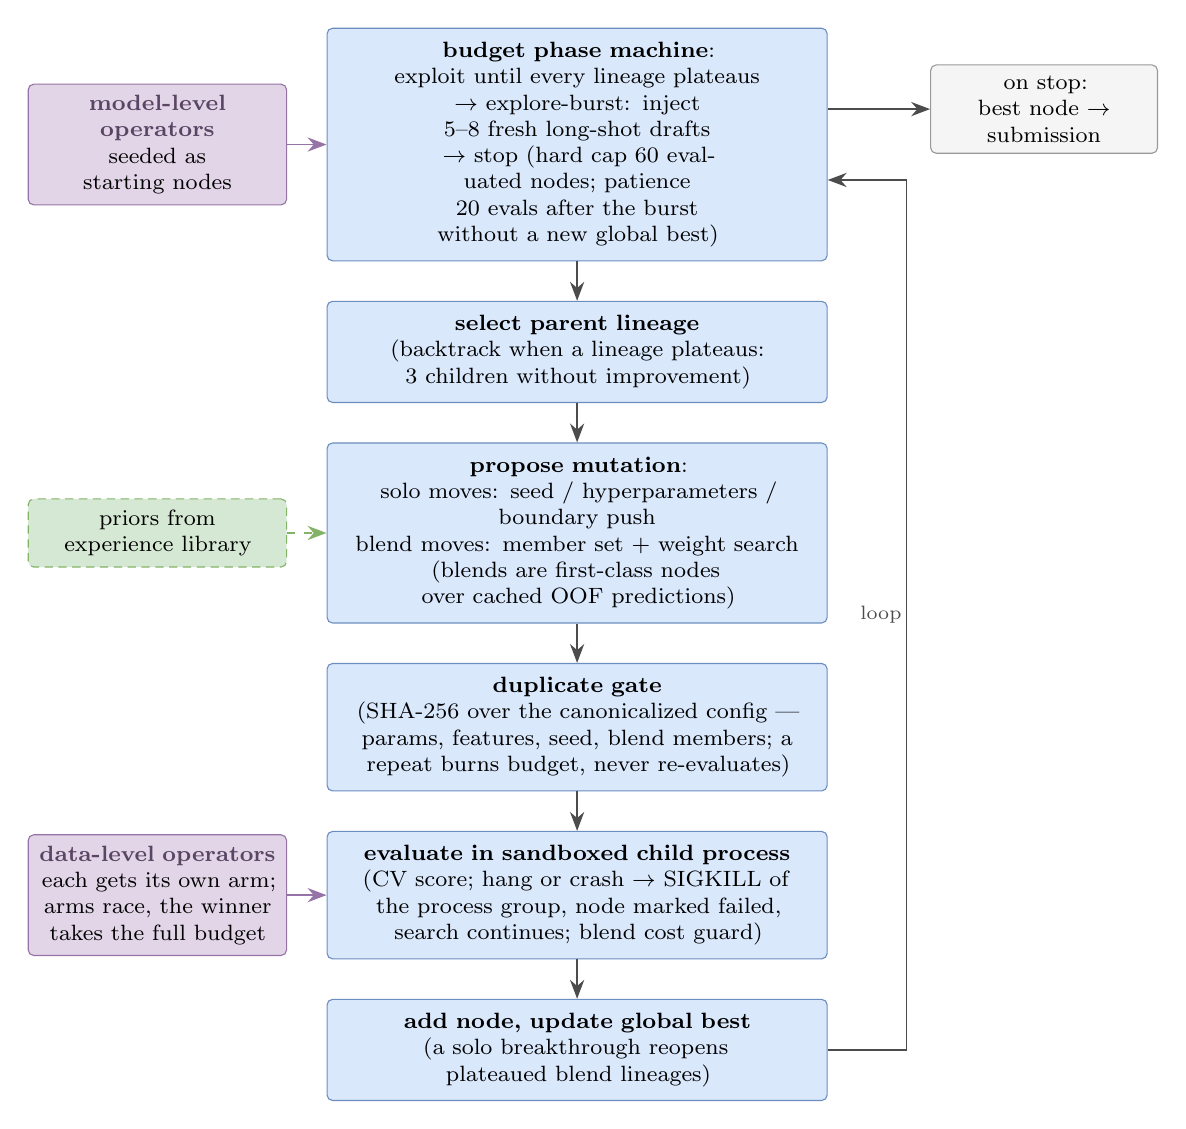
\begin{tikzpicture}[
  font=\footnotesize,
  sbox/.style={draw=flowblueline, rounded corners=2pt, align=center, inner sep=5pt,
               fill=flowblue, text width=60mm},
  sidebox/.style={draw=flowgreyline, rounded corners=2pt, align=center, inner sep=4pt,
                  fill=flowgrey, text width=30mm},
  injside/.style={sidebox, fill=flowpurple, draw=flowpurpleline},
  priorbox/.style={sidebox, fill=flowgreen, draw=flowgreenline, densely dashed},
  arr/.style={-{Stealth[length=2.4mm]}, semithick, black!70},
  parr/.style={arr, flowpurpleline},
  darr/.style={arr, dashed},
  lab/.style={font=\scriptsize, inner sep=1.5pt},
  node distance=5mm
]
% ----- main loop column -----
\node[sbox] (phase) {\textbf{budget phase machine}:\\exploit until every lineage plateaus\\$\to$ explore-burst: inject 5--8 fresh long-shot drafts\\$\to$ stop (hard cap 60 evaluated nodes; patience\\20 evals after the burst without a new global best)};
\node[sbox, below=of phase] (select) {\textbf{select parent lineage}\\(backtrack when a lineage plateaus: 3 children without improvement)};
\node[sbox, below=of select] (propose) {\textbf{propose mutation}:\\solo moves: seed / hyperparameters /\\boundary push\\blend moves: member set + weight search\\(blends are first-class nodes over cached OOF predictions)};
\node[sbox, below=of propose] (dedup) {\textbf{duplicate gate}\\(SHA-256 over the canonicalized config --- params, features, seed, blend members; a repeat burns budget, never re-evaluates)};
\node[sbox, below=of dedup] (eval) {\textbf{evaluate in sandboxed child process}\\(CV score; hang or crash $\to$ SIGKILL of the process group, node marked failed, search continues; blend cost guard)};
\node[sbox, below=of eval] (add) {\textbf{add node, update global best}\\(a solo breakthrough reopens plateaued blend lineages)};
\foreach \a/\b in {phase/select, select/propose, propose/dedup, dedup/eval, eval/add}{\draw[arr] (\a) -- (\b);}
% ----- loop back, right side -----
\draw[arr] (add.east) -- ++(10mm,0) |- node[lab, pos=0.25, left]{loop} ([yshift=-4.5mm]phase.east);
% ----- exit, top right -----
\node[sidebox, text width=26mm, anchor=west] (out) at ([xshift=13mm, yshift=4.5mm]phase.east)
  {on stop:\\best node $\to$ submission};
\draw[arr] ([yshift=4.5mm]phase.east) -- (out.west);
% ----- side inputs, left column -----
\node[injside, left=5mm of phase] (injcfg)
  {\textcolor{flowpurpleline!60!black}{\textbf{model-level operators}}\\seeded as\\starting nodes};
\draw[parr] (injcfg) -- (phase);
\node[priorbox, left=5mm of propose] (prior)
  {priors from\\experience library};
\draw[darr, flowgreenline] (prior) -- (propose);
\node[injside, left=5mm of eval] (injdata)
  {\textcolor{flowpurpleline!60!black}{\textbf{data-level operators}}\\each gets its own arm; arms race, the winner takes the full budget};
\draw[parr] (injdata) -- (eval);
\end{tikzpicture}
\caption{The tree-search loop used in all my-agent runs of this report (37--224 nodes per
competition; per-competition counts in Table~\ref{tab:nodes}). Each node is a complete,
executable solution scored by local cross-validation; lineages are abandoned on plateau, and
the budget phase machine forces one exploration burst before stopping. Figure~\ref{fig:treeex} shows what the
loop builds. Purple: the injection
layer's operator entry points (Section~\ref{sec:v5}) --- model-level operators seed starting
nodes; data-level operators build separately raced arms. Green: priors from the experience
library. Solid arrows: the loop's execution flow; dashed: advisory input and backtracking.}
\label{fig:tree}
\end{figure}

\begin{figure}[htbp]
\centering
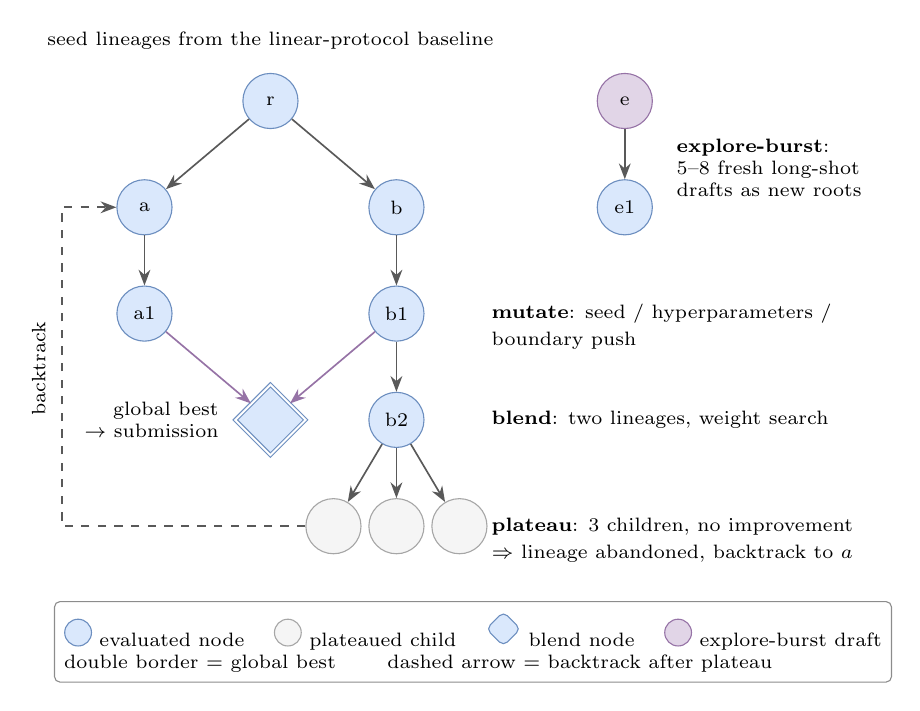
\begin{tikzpicture}[
  font=\footnotesize,
  tn/.style={circle, draw=flowblueline, fill=flowblue, inner sep=0pt, minimum size=7mm,
             font=\scriptsize},
  bn/.style={tn, draw=flowpurpleline, fill=flowpurple},
  pl/.style={tn, draw=black!35, fill=flowgrey, text=black!45},
  bl/.style={tn, diamond, minimum size=9mm},
  te/.style={-{Stealth[length=2mm]}, semithick, black!65},
  lab/.style={font=\scriptsize, inner sep=1.5pt}
]
% ----- lineage a and lineage b, grown from the root -----
\node[tn] (r)  at (3.1,0)     {r};
\node[tn] (A)  at (1.5,-1.35)  {a};
\node[tn] (B)  at (4.7,-1.35)  {b};
\node[tn] (A1) at (1.5,-2.7)   {a1};
\node[tn] (B1) at (4.7,-2.7)   {b1};
\node[tn] (B2) at (4.7,-4.05)  {b2};
\node[pl] (c1) at (3.9,-5.4)   {};
\node[pl] (c2) at (4.7,-5.4)   {};
\node[pl] (c3) at (5.5,-5.4)   {};
% ----- blend node = global best -----
\node[bl, double, double distance=0.7pt] (bd) at (3.1,-4.05) {};
% ----- explore-burst draft as a new root -----
\node[bn] (e)  at (7.6,0)      {e};
\node[tn] (e1) at (7.6,-1.35)  {e1};
\foreach \a/\b in {r/A, r/B, A/A1, B/B1, B1/B2, B2/c1, B2/c2, B2/c3, e/e1}{\draw[te] (\a) -- (\b);}
\draw[te, flowpurpleline] (B1) -- (bd);
\draw[te, flowpurpleline] (A1) -- (bd);
% ----- backtrack: the plateaued lineage is abandoned -----
\draw[te, dashed] (c1.west) -- (0.45,-5.4) -- (0.45,-1.35) -- (A.west);
\node[lab, rotate=90, anchor=south] at (0.3,-3.4) {backtrack};
% ----- annotations -----
\node[lab, anchor=south] at (3.1,0.6)   {seed lineages from the linear-protocol baseline};
\node[lab, anchor=west] at (5.85,-2.7)  {\textbf{mutate}: seed / hyperparameters /};
\node[lab, anchor=west] at (5.85,-3.05) {boundary push};
\node[lab, anchor=west] at (5.85,-4.05) {\textbf{blend}: two lineages, weight search};
\node[lab, anchor=west] at (5.85,-5.4)  {\textbf{plateau}: 3 children, no improvement};
\node[lab, anchor=west] at (5.85,-5.75) {$\Rightarrow$ lineage abandoned, backtrack to $a$};
\node[lab, anchor=west, align=left] at (8.2,-0.85) {\textbf{explore-burst}:\\5--8 fresh long-shot\\drafts as new roots};
\node[lab, anchor=east, align=right] at (2.5,-4.05) {global best\\$\to$ submission};
% ----- legend -----
\node[draw=black!45, rounded corners=2pt, inner sep=3.5pt, anchor=north west,
      align=left, font=\scriptsize] at (0.35,-6.35)
  {\tikz\node[tn, minimum size=3.4mm]{};~evaluated node \quad
   \tikz\node[pl, minimum size=3.4mm]{};~plateaued child \quad
   \tikz\node[bl, minimum size=4.4mm]{};~blend node \quad
   \tikz\node[bn, minimum size=3.4mm]{};~explore-burst draft\\
   double border~$=$~global best \qquad dashed arrow~$=$~backtrack after plateau};
\end{tikzpicture}
\caption{What my-agent's tree search builds: one search tree, schematic (the search loop
itself is Fig.~\ref{fig:tree}). Each node is a complete, executable solution scored by local
cross-validation. Two lineages grow from the linear-protocol baseline; lineage $b$ plateaus
after three children fail to improve, so the search backtracks and abandons it; a blend node
over the cached out-of-fold predictions of $a1$ and $b1$ becomes the global best and is what
gets submitted; the forced explore-burst injects fresh long-shot drafts ($e$) as new roots.
Node labels are schematic --- real runs evaluate 37--224 nodes per competition
(Table~\ref{tab:nodes}).}
\label{fig:treeex}
\end{figure}

\begin{table}[htbp]
\centering\small
\caption{Evaluated tree-search nodes per competition (my-agent), from each completed
benchmark lane's search records (\texttt{experiments\_tree\_v3.json} / lane \texttt{STATUS.md}).
The default budget is 60 evaluated nodes; lanes may extend it through the documented
\texttt{extend\_budget} resume path (s3e9, s4e11, tps-aug-2022); conway stopped at 37 on the
wall-clock backstop; s5e1's count sums its six separately raced external-data arms;
tps-jan-2022 is the clean re-run (81 nodes over two rounds).}
\label{tab:nodes}
\begin{tabular}{@{}lr@{\hspace{2em}}lr@{\hspace{2em}}lr@{}}
\toprule
\textbf{Competition} & \textbf{Nodes} & \textbf{Competition} & \textbf{Nodes} & \textbf{Competition} & \textbf{Nodes} \\
\midrule
s3e1 & 53 & s3e16 & 45 & s6e1 & 47 \\
s3e3 & 60 & s3e19 & 60 & s6e2 & 57 \\
s3e5 & 60 & s4e11 & 110 & afsis & 60 \\
s3e7 & 49 & s5e1 & 224$^{\ast}$ & cat-in-the-dat & 70 \\
s3e9 & 107 & s5e10 & 46 & conway & 37 \\
s3e11 & 60 & & & tps-aug-2022 & 126 \\
s3e14 & 70 & & & tps-jan-2022 & 81 \\
      &    & & & tps-sep-2022 & 60 \\
\bottomrule
\end{tabular}

\smallskip
\raggedright\footnotesize $^{\ast}$~Six separately raced external-data arms
($30+60+30+14+60+30$), the arms-race design of Section~\ref{sec:v5}.
\end{table}

\FloatBarrier

\subsection{Isolation protocol and design comparison}

Table~\ref{tab:fairness} names the four isolation conditions of the fairness protocol together
with what enforces each; the Methods state the conditions themselves.
Table~\ref{tab:threeway} sets the three methods side by side on the axes that separate them.

\begin{table}[htbp]
\centering\small
\caption{The four isolation conditions and what enforces each.}
\label{tab:fairness}
\begin{tabular}{@{}L{2.6cm}L{6.4cm}L{5.6cm}@{}}
\toprule
\textbf{Condition} & \textbf{Rule} & \textbf{Enforcement} \\
\midrule
Data & Each side reads only its own root, containing files validated against the official Kaggle manifest & \path{build_isolated_roots.py} \\
Workspace & The three output directories are fully separated; each side is scored independently & Directory structure \\
Instruction & Prompts may carry environment facts and metric thresholds only --- no modelling recipes, no other side's scores, no workaround discovered by another side & Manual protocol + incident log \\
Resource & Only one lane executes at any moment & \path{lane_lock.sh} mutex \\
\bottomrule
\end{tabular}
\end{table}

\begin{table}[htbp]
\centering\footnotesize
\setlength{\tabcolsep}{4pt}
\caption{Design comparison of the three methods.}
\label{tab:threeway}
\begin{tabular}{@{}L{3.2cm}L{4.2cm}L{3.4cm}L{3.6cm}@{}}
\toprule
\textbf{Aspect} & \textbf{my-agent} & \textbf{AIDE} & \textbf{NVIDIA} \\
\midrule
Knowledge source & Cross-competition experience library (accumulating) & None (from zero each time) & Public kernels fetched fresh each time \\
Search strategy & Six-stage pipeline + tree search (37--224 nodes) & Tree-shaped trial and error, 20 steps & No search; faithful reproduction \\
Basis for next step & Experience-library priors + OOF diagnostics & Previous step's error or score & Highest-voted kernel \\
Validation rigor & Split chosen by task type; diagnostics tagged and excluded & No concept of split legality & Inherits the kernel's split \\
External data & Injection layer (typed operators, whitelisted sources) & Never considered & Inherited from the kernel \\
\bottomrule
\end{tabular}
\end{table}

\FloatBarrier

\subsection{Cross-competition rule: split strategy is determined by task type}

Every lane chooses its validation split from the task type alone, by the rule of
Table~\ref{tab:splits}, before any score is seen.

\begin{table}[H]
\centering\small
\caption{Validation-split policy by task type.}
\label{tab:splits}
\begin{tabular}{@{}L{4.2cm}L{4.4cm}L{6.0cm}@{}}
\toprule
\textbf{Task type} & \textbf{Required split} & \textbf{Rationale} \\
\midrule
Time-series extrapolation (test set later than training period) & Time-based split (\texttt{year < y} vs \texttt{year == y}) or TimeSeriesSplit & Each validation block must be strictly later than its training window, mirroring the true train--test gap \\
Text pairing (same anchor in many rows) & GroupKFold by anchor & Otherwise one anchor spans train and validation, and the model memorizes anchors instead of semantic relations \\
Generic tabular (continuous i.i.d.\ target) & Shuffled KFold / StratifiedKFold & No temporal or group structure \\
\bottomrule
\end{tabular}
\end{table}

Shuffled KFold on time-series data is strictly forbidden: on s3e19 this one error cost AIDE a
$4.5\times$ optimism bias, while my-agent quarantined the same split as diagnostic
(Section~\ref{sec:exp4}).

\subsection{Execution environment}

Table~\ref{tab:env} records the environment items the fairness protocol
(Section~\ref{sec:fairness}) does not state.

\begin{table}[H]
\centering\small
\caption{Execution environment.}
\label{tab:env}
\begin{tabular}{@{}L{3.6cm}L{10.8cm}@{}}
\toprule
\textbf{Item} & \textbf{Detail} \\
\midrule
Hardware & ARM64 Linux (Ubuntu 24.04), NVIDIA GB10 GPU \\
Environment management & uv + \texttt{uv.lock} (frozen versions); Python 3.13 \\
Monitoring & \texttt{bench-watchdog.timer}, checking every 15 minutes for (a) machine idle with work pending, (b) process alive but no output for 30 minutes, (c) individual driver death \\
Determinism & Fixed seeds; LightGBM with \texttt{deterministic=true}, \path{force_row_wise=true}, fixed \path{num_threads} --- necessary for cross-process reproducibility \\
Per-step memory cap & 32 GB (exceeding it marks the node buggy; a single step once consumed 76 GB and stalled the machine) \\
Output isolation & my-agent \path{kaggle/competitions/}; AIDE \path{aideml-runs/}; NVIDIA \path{nvidia-kaggle-runs/} \\
\bottomrule
\end{tabular}
\end{table}

\subsection{Cross-competition rule: deep-learning-to-GBDT field mapping}

The specification framework of the companion per-competition reports carries several
deep-learning-specific fields; this study is GBDT-centric, and every GBDT report maps them as in
Table~\ref{tab:dlgbdt}.

\begin{table}[H]
\centering\small
\caption{Mapping of deep-learning framework fields to their GBDT counterparts.}
\label{tab:dlgbdt}
\begin{tabular}{@{}L{4.6cm}L{9.8cm}@{}}
\toprule
\textbf{Framework field} & \textbf{GBDT counterpart} \\
\midrule
Learning Rate & Boosting shrinkage (\path{learning_rate}) \\
Learning Rate Scheduler & N/A --- convergence governed by CV early stopping, not a schedule \\
Batch Size & N/A --- full-dataset histogram boosting, not mini-batches \\
Model Complexity & Expressed as ``number of trees $\times$ leaves,'' not dense parameter count \\
Transfer Learning & N/A (no pretrained weights); analogue: prior injection from the experience library \\
Data Augmentation & N/A (tabular); analogue: feature engineering and seed bagging \\
\bottomrule
\end{tabular}
\end{table}

\FloatBarrier

\subsection{Per-competition specification reports}
\label{app:specs}

The pipeline documents its own work. Each competition receives a specification report written to
the five sections of Tso-Jung Yen's ML specification framework (\path{ml_pipeline_modules}) ---
Data / Models \& Architecture / Training / Inference / Evaluation \& Benchmarking: 22 reports for
my-agent, covering the 20 benchmark competitions plus two development-lane competitions
(\path{docs/ml_specs/}, MD + PDF), and 17 re-documenting the AIDE runs under the same framework
(\path{benchmark_results/ml_specs_aide/}, MD + PDF). Every number in them is extracted
deterministically by \texttt{collect.py} and \path{collect_aide_facts.py} from that competition's
structured records --- \texttt{facts.json}, \path{eda_summary.json},
\path{experiments_tree_v3.json}, \path{journal.json} --- and never generated by an LLM; a field
the records do not contain is printed as ``not recorded'' rather than left blank or estimated.
The my-agent set ships \texttt{RUBRIC.md}, an 8-item plan-alignment checklist verified per
competition, and all 22 reports pass 8/8. The structured EDA pass each lane records ---
distributions, drift, correlation, written to \path{eda_summary.json} and
\path{eda_output.txt}, with no image files emitted --- is one of the sources these reports read.
The reports are CV-only by construction, so their conclusions must not be mixed with the
leaderboard verdicts of the main text.

\subsection{Companion documents}
\label{app:coverage}

Two companion documents carry material that answers questions this paper does not.
\emph{Building the Injection Layer: An Engineering Log} is written for someone rebuilding a
similar system: it holds the per-regime coverage tables behind the consumer trace of
Section~\ref{sec:exp6v5} together with the audit scripts that reproduce them; the record of every
occasion one of the isolation mechanisms of Table~\ref{tab:fairness} failed, what it cost and how
it was caught; the minute-by-minute reconstruction of the voided ventilator attempt; and the nine
defects found in a single day's audit of the injection layer --- six from the audit itself, three
from verifying the fixes for the first six. \emph{Per-Competition Case Studies} carries the
single-competition forensic depth: the CV--leaderboard reversal mechanics, AIDE's step-by-step
split switch, the two experience-library entries behind the midterm correction, the s5e1 setting
behind the pre-registered prediction, and the s3e19 residual decomposition in full.

\subsection{Minimal steps to reproduce a lane}

Paths are relative to the project repository named in Methods, in which infrastructure scripts
that live above the agent directory are mirrored under \path{benchmark_infra/}.

\begin{verbatim}
# 1) Build isolated data roots (per official Kaggle manifest)
python benchmark_infra/build_isolated_roots.py --write <comp>

# 2) my-agent, one competition
cd ai_agents/kaggle && claude -p "<see run_myagent_headless.sh PROMPT>" \
    --dangerously-skip-permissions

# 3) AIDE, one competition (20 steps)
AIDE_COMP_ROOT=<data-root> \
    python benchmark_infra/run_comp.py <comp> --shim --steps 20

# 4) NVIDIA, one competition
python benchmark_infra/run_ready_reproductions.py

# 5) Submit and retrieve public/private scores
KAGGLE_API_TOKEN=$(cat ~/.kaggle/huang_token) \
    kaggle competitions submit -c <comp> \
    -f submission.csv -m "<msg>"
\end{verbatim}

Environment: ARM64 Linux (Ubuntu 24.04), NVIDIA GB10 GPU, uv-managed Python 3.13, versions frozen
in \texttt{uv.lock}.

% ---------------------------------------------------------------------
% References (kept after the appendix, outside the counted body).
% MAINTAINER: delete this block if the bibliography is supplied elsewhere.
% ---------------------------------------------------------------------
\begin{thebibliography}{9}
\bibitem{aygun2026} Ayg\"un, E., et al. An AI system to help scientists write expert-level empirical software. \emph{Nature} (2026). \url{https://doi.org/10.1038/s41586-026-10658-6}
\bibitem{aide2025} Jiang, Z., Schmidt, D., Srikanth, D., Xu, D., Kaplan, I., Jacenko, D., and Wu, Y. AIDE: AI-Driven Exploration in the Space of Code. arXiv:2502.13138 (2025).
\bibitem{nvidia2026} NVIDIA. Kaggle Agent: kernel-reproduction agent skill (software), 2026.
\bibitem{mlebench} Chan, J.\,S., et al. MLE-bench: Evaluating Machine Learning Agents on Machine Learning Engineering. arXiv:2410.07095 (2024).
\end{thebibliography}


\end{document}
